\documentclass[12pt,t]{beamer}
\usepackage[brazil]{babel}
\usepackage[utf8x]{inputenc}
\usepackage{beamerthemeboadilla}
\usepackage[alf]{abntex2cite}	
\usepackage{tabulary}
\usepackage{tabularx} 
\usepackage{booktabs}
\usepackage{multirow}
\usepackage{caption}
\usepackage{graphicx}
\usepackage{epstopdf}
\usepackage{etoolbox}
\usepackage{mathabx}
\usepackage{url}
\usepackage{listings}

\usepackage[framemethod=tikz]{mdframed}

\lstset{language=Java,
        basicstyle=\scriptsize,
        keywordstyle=\scriptsize\color{blue},
        commentstyle=\color{green},
	    stringstyle=\color{magenta},
        showstringspaces=false
}

\usepackage[htt]{hyphenat}
\usepackage{etoolbox}
\usepackage[abs]{overpic}

\usepackage{tikz}

\usepackage[euler]{textgreek}

\usepackage{changepage}

\usetikzlibrary{shapes.geometric, arrows}

\newcommand\eqdef{\mathrel{\overset{\makebox[0pt]{\mbox{\normalfont\tiny\sffamily def}}}{=}}}

\defbeamertemplate{description item}{align left}{\insertdescriptionitem\hfill}

\institute{POO 2015\\IME -- USP}
\author{Bruno Sofiato\\Vinicius Nascimento Silva}

\title{Reflexão computacional e meta-objetos}

\makeatletter
\patchcmd{\beamer@sectionintoc}
{\vfill}
{\vskip\itemsep}
{}
{}
\makeatother  
%\usepackage{default}

\AtBeginSection[]{
	\begin{frame}[c]{ }
		\centering
		\begin{beamercolorbox}[sep=8pt,center,shadow=true,rounded=true]{title}
			\huge\insertsectionhead\par%
		\end{beamercolorbox}
	\end{frame}
}


\begin{document}
\abovedisplayskip=0pt
\abovedisplayshortskip=0pt
\belowdisplayskip=0pt
\belowdisplayshortskip=0pt	
 \frame{\titlepage}
 \begin{frame}{Agenda}
	\tableofcontents
 \end{frame}
 \section{Objetivos}
 \begin{frame}{Objetivos}
 	\begin{block}{Objetivos}
 		\begin{itemize}
 			\item Explicar os conceitos relativos a meta-objetos e linguagens reflexivas;
 			\pause
 			\item Mostrar um panorama das característica reflexivas das linguagens de programação;
 			\pause
 			\item Exemplificar usos de reflexão.
 		\end{itemize}
 	\end{block}
 	\pause
 	\begin{block}{Escopo}
 		Linguagens orientadas a objetos baseadas em classes, segundo categorização de \citeonline{wegner1987dimensions} (\emph{Dimensions of object-based language design}).
 	\end{block}
 \end{frame}
 \section{Meta-modelo}
	 \begin{frame}{Meta-}
	 	\begin{block}{Etimologia}
	 		O prefixo meta- remete ao grego μετα, que significa \emph{além} ou \emph{depois}.
	 	\end{block}
	 	\pause
	 	\begin{block}{Significado}
	 		Geralmente é usado para representar um conceito que é uma abstração de outro.
	 	\end{block}
	 	\pause
	 	\begin{exampleblock}{Exemplos}
	 		\begin{description}[Metalinguagem]
	 			\item [Metafísica] É a investigação das realidades que transcendem a experiência sensível.
	 			\item [Metalinguagem] São linguagens utilizadas para definição de outras linguagens:
	 			\begin{itemize}
	 				\item EBNF 
	 				\item XML (schema)
	 			\end{itemize}
	 		\end{description}
	 	\end{exampleblock}
	 	\end{frame}
	 	\begin{frame}{Metamodelos}
	 		\begin{block}{Definição}
	 			Informalmente é um modelo de um modelo.
	 		\end{block}
	 		\pause
	 		\begin{block}{Usos}
	 			Normalmente, são utilizados em ferramentas que oferecem suporte à criação de modelos. Entre elas, ferramentas de CAD, CAE e CASE.
	 		\end{block}
	 		\pause
	 		\begin{exampleblock}{Exemplos}
	 			\begin{description}[Datawarehousing]
	 			\item [Construção Civil] \emph{Building Information Model} (BIM);
	 			\item [Datawarehousing]		
	 		\emph{Common Warehouse MetaModel} (CWM);
	 			\item [Matemática] Teoria das Categorias;
	 			\item [Programas OO] \emph{Unified Modeling Language} (UML).
	 		\end{description}
		\end{exampleblock}
	 \end{frame}
	 \begin{frame}{MOF -- Meta-object Facility}
	 	\begin{block}{Características}
	 		\begin{itemize}
	 			\item Definida pela OMG (Object Management Group) para a modelagem de metamodelos (versão atual -- 2.4.2);
	 		\end{itemize}
	 	\end{block}	 
	 	\begin{block}{ }
 	 		\centerline{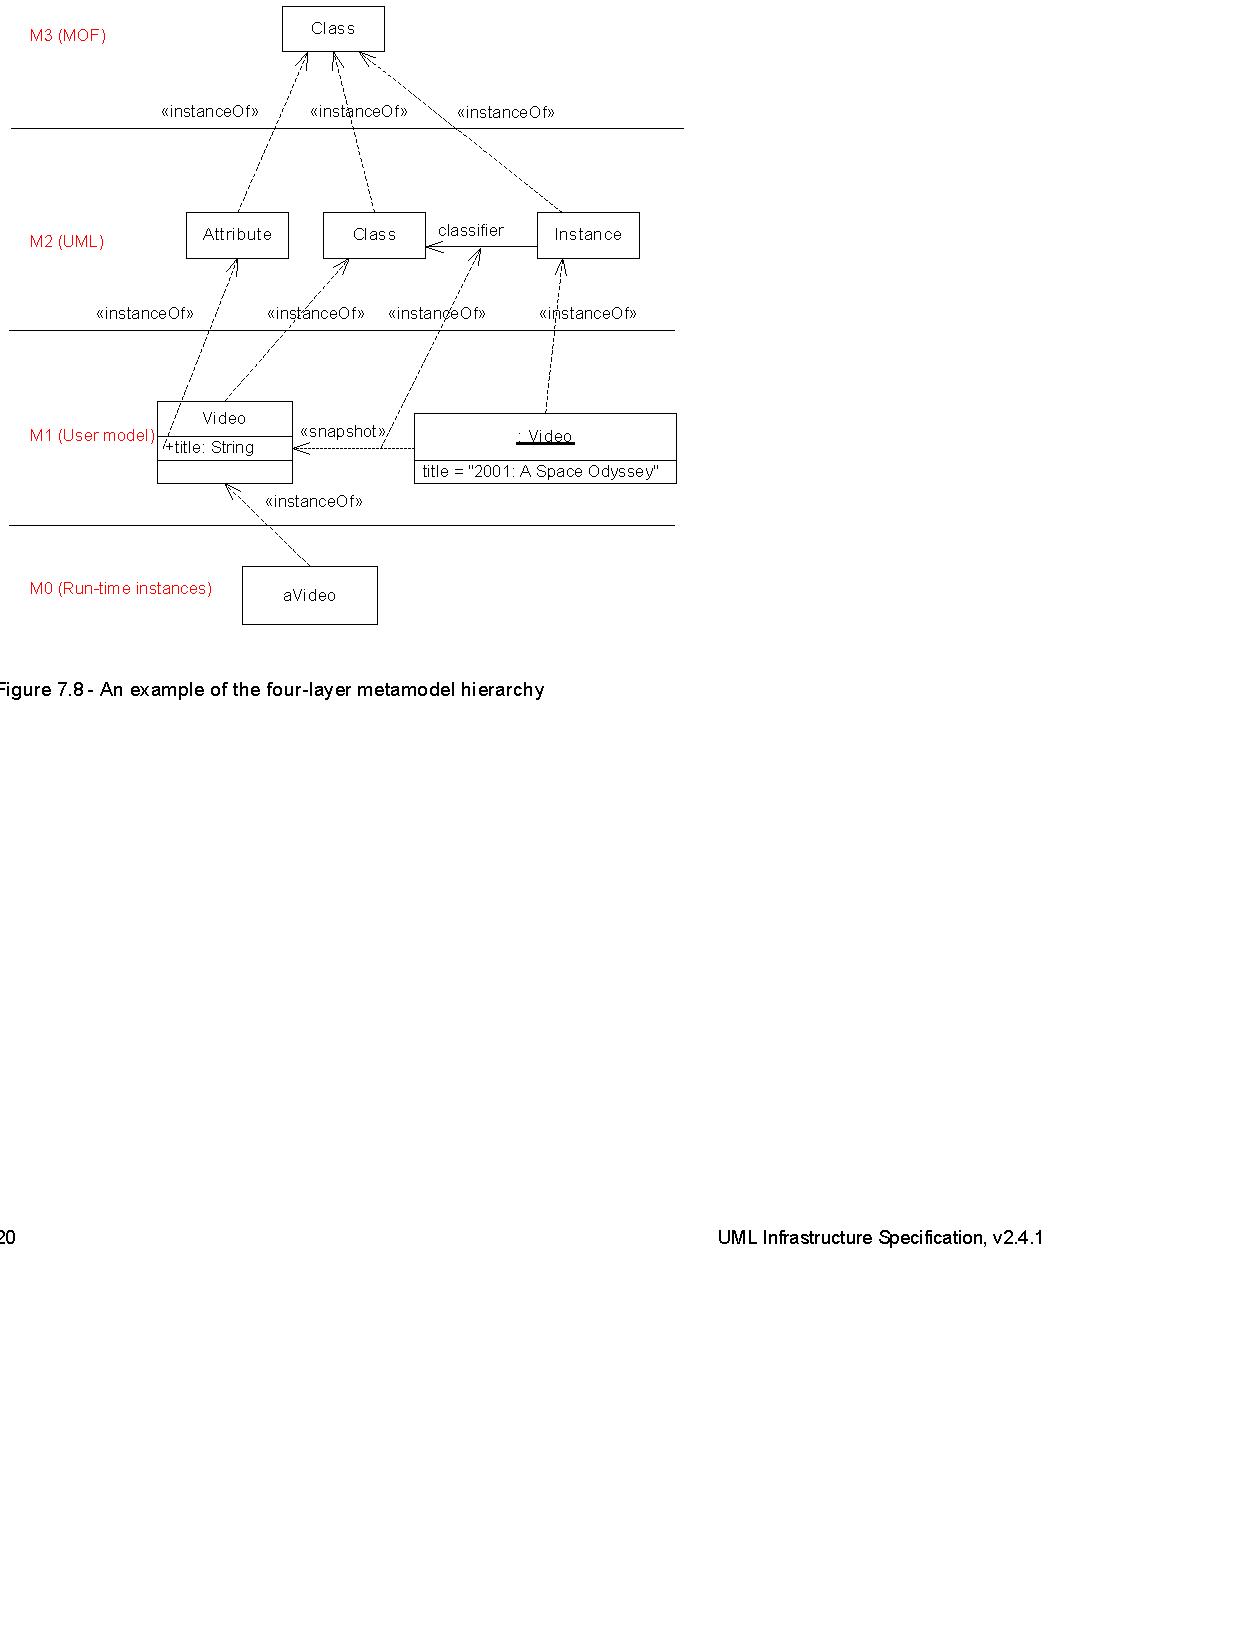
\includegraphics[trim=0 430 260 5, clip=true, totalheight=0.80\textheight]{mof.pdf}}
	 	\end{block}
     \end{frame}
	 \begin{frame}{Meta-modelo UML}
	 	\begin{block}{Características}
	 		\begin{itemize}
	 			\item Mantido pela OMG, define a estrutura e a semântica dos construtos da UML (versão atual -- 2.4.2);
	 			\pause
	 			\item Incluso na 2a camada MOF;
	 		\end{itemize}
	 	\end{block}
	 	\begin{block}{ }
 	 		\centerline{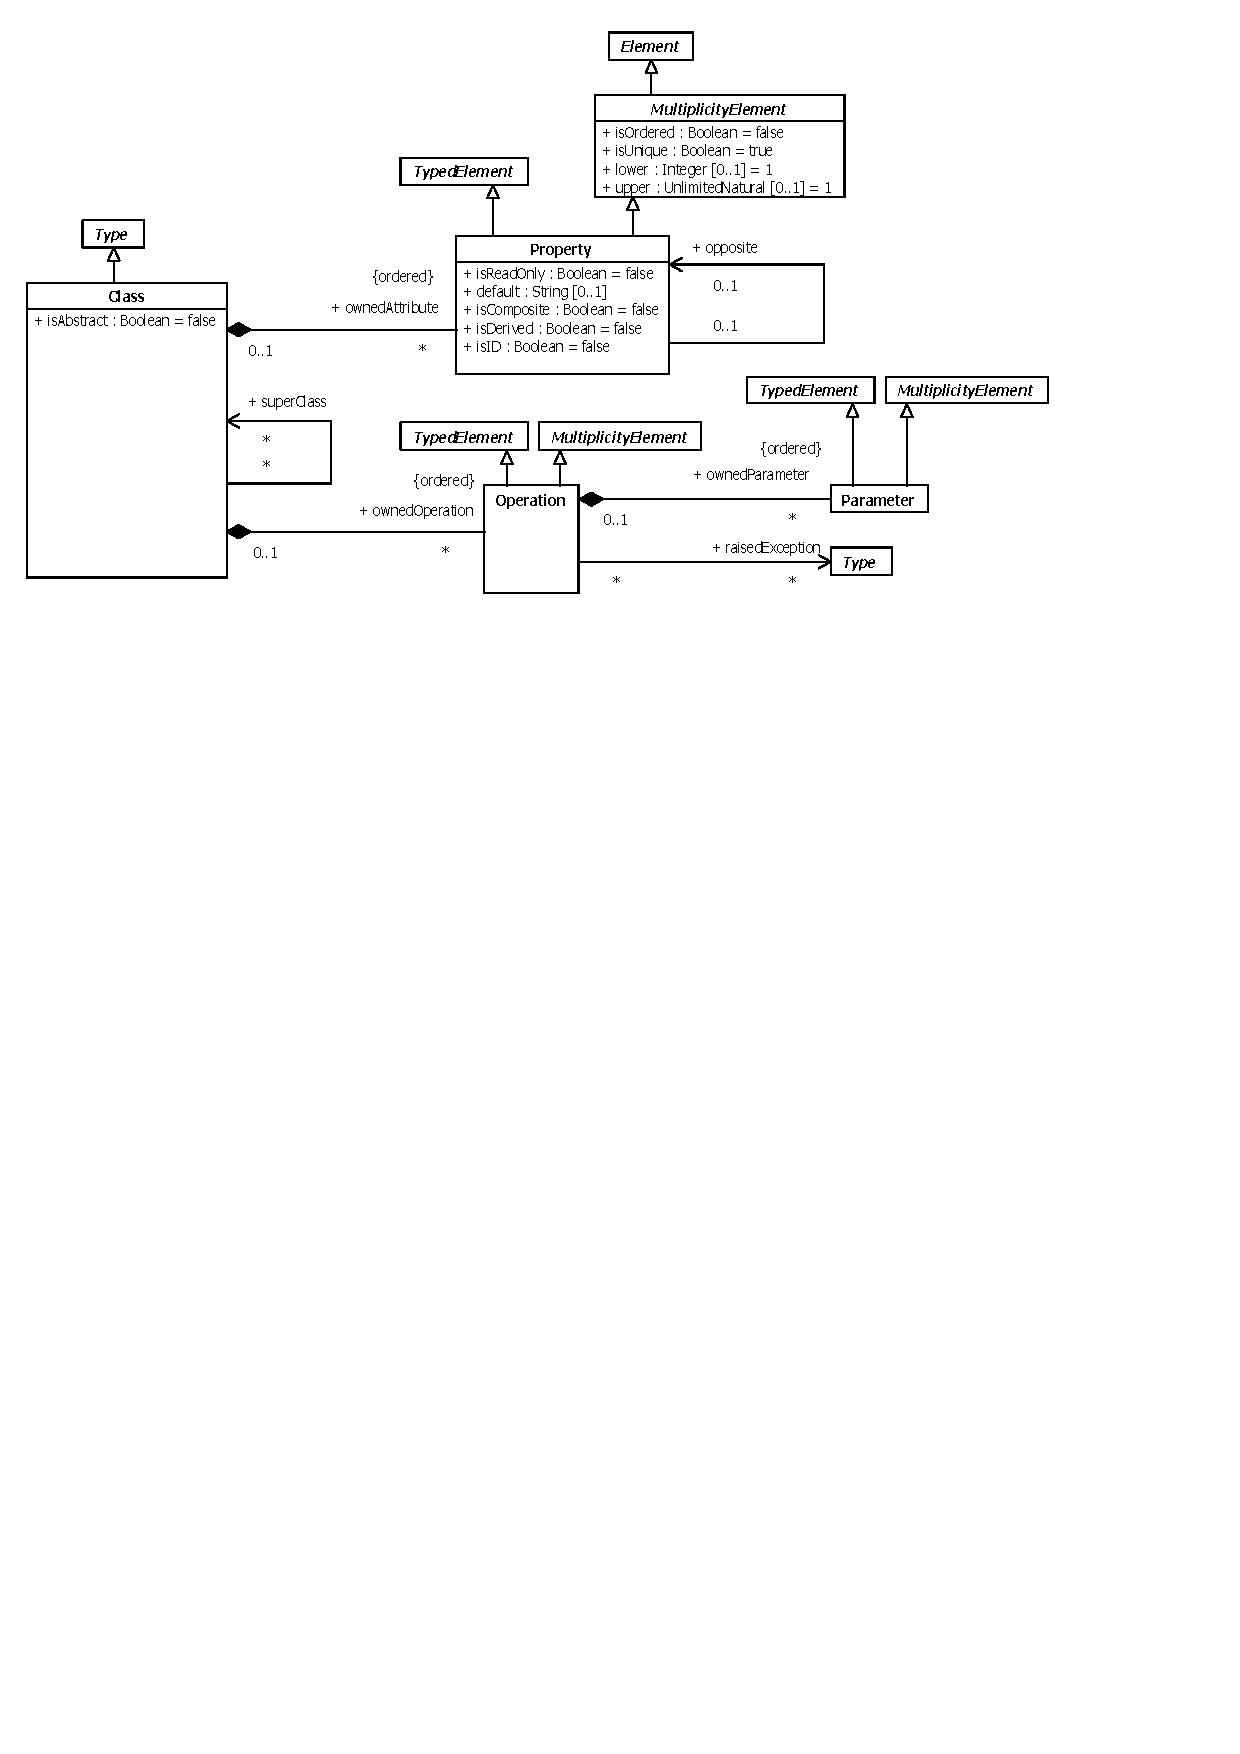
\includegraphics[trim=10 430 70 15, clip=true, height=0.80\textheight]{uml.pdf}}
	 	\end{block}
	\end{frame}	 	
	% \begin{frame}[c]{ }
	%	\centering
	%	\LARGE E se esse modelo estivesse disponível em tempo de execução ?
	% \end{frame}
 \section{Programação Reflexiva}
	 \begin{frame}{O que é reflexão}
	 	\begin{block}{Definição}
	 		\begin{quote}
				It's all about building your language out of first-class, dynamic object that you can look at and change at runtime.
	 		\begin{flushright}
	 			Brian Foote
	 		\end{flushright} 	 		
	 		\end{quote}
	 	\end{block}
	 	\pause
	 	\begin{block}{História}
	 		\begin{description}[9999]
	 			\item[1982] Definição por \citeonline{smith1982reflection} das características de sistemas ditos reflexivos;
	 			\item[1983] Smalltalk-80 incorpora a noção classes sendo objetos -- podendo assim responder à mensagens;
	 			\item[1984] \citeonline{friedman1984reification} descrevem um mecanismo que permite a criação de sistemas reflexivos;
	 			\item[1991] \citeonline{kiczales1991art} escreve o livro \emph{The Art of Metaobject Protocol}.
	 		\end{description}
	 	\end{block}	
	 \end{frame}
	 \begin{frame}{Procedural reflection in programming languages \cite{smith1982reflection}}
	 	\begin{block}{Descrição}
	 		Define as três caraterísticas básicas necessárias em sistemas reflexivos. 
	 	\end{block}
	 	\pause
	 	\begin{block}{Características -- Sistemas Reflexivos}
	 	  \begin{enumerate}
	 	  	\item Um sistema deve ter uma representação de si mesmo;
	 	  	\pause
	 	  	\item Deve haver uma conexão causal entre um sistema e sua representação;
	 	  	\pause
	 	  	\item Devem existir mecanismos com os quais um programa pode manipular sua representação. 
	 	  \end{enumerate}
	 	\end{block}
	 \end{frame}
	 \begin{frame}{Reification -- Reflection without Metaphysics \cite{friedman1984reification}}
	 	\begin{block}{ }
 	 		\centering
 	 		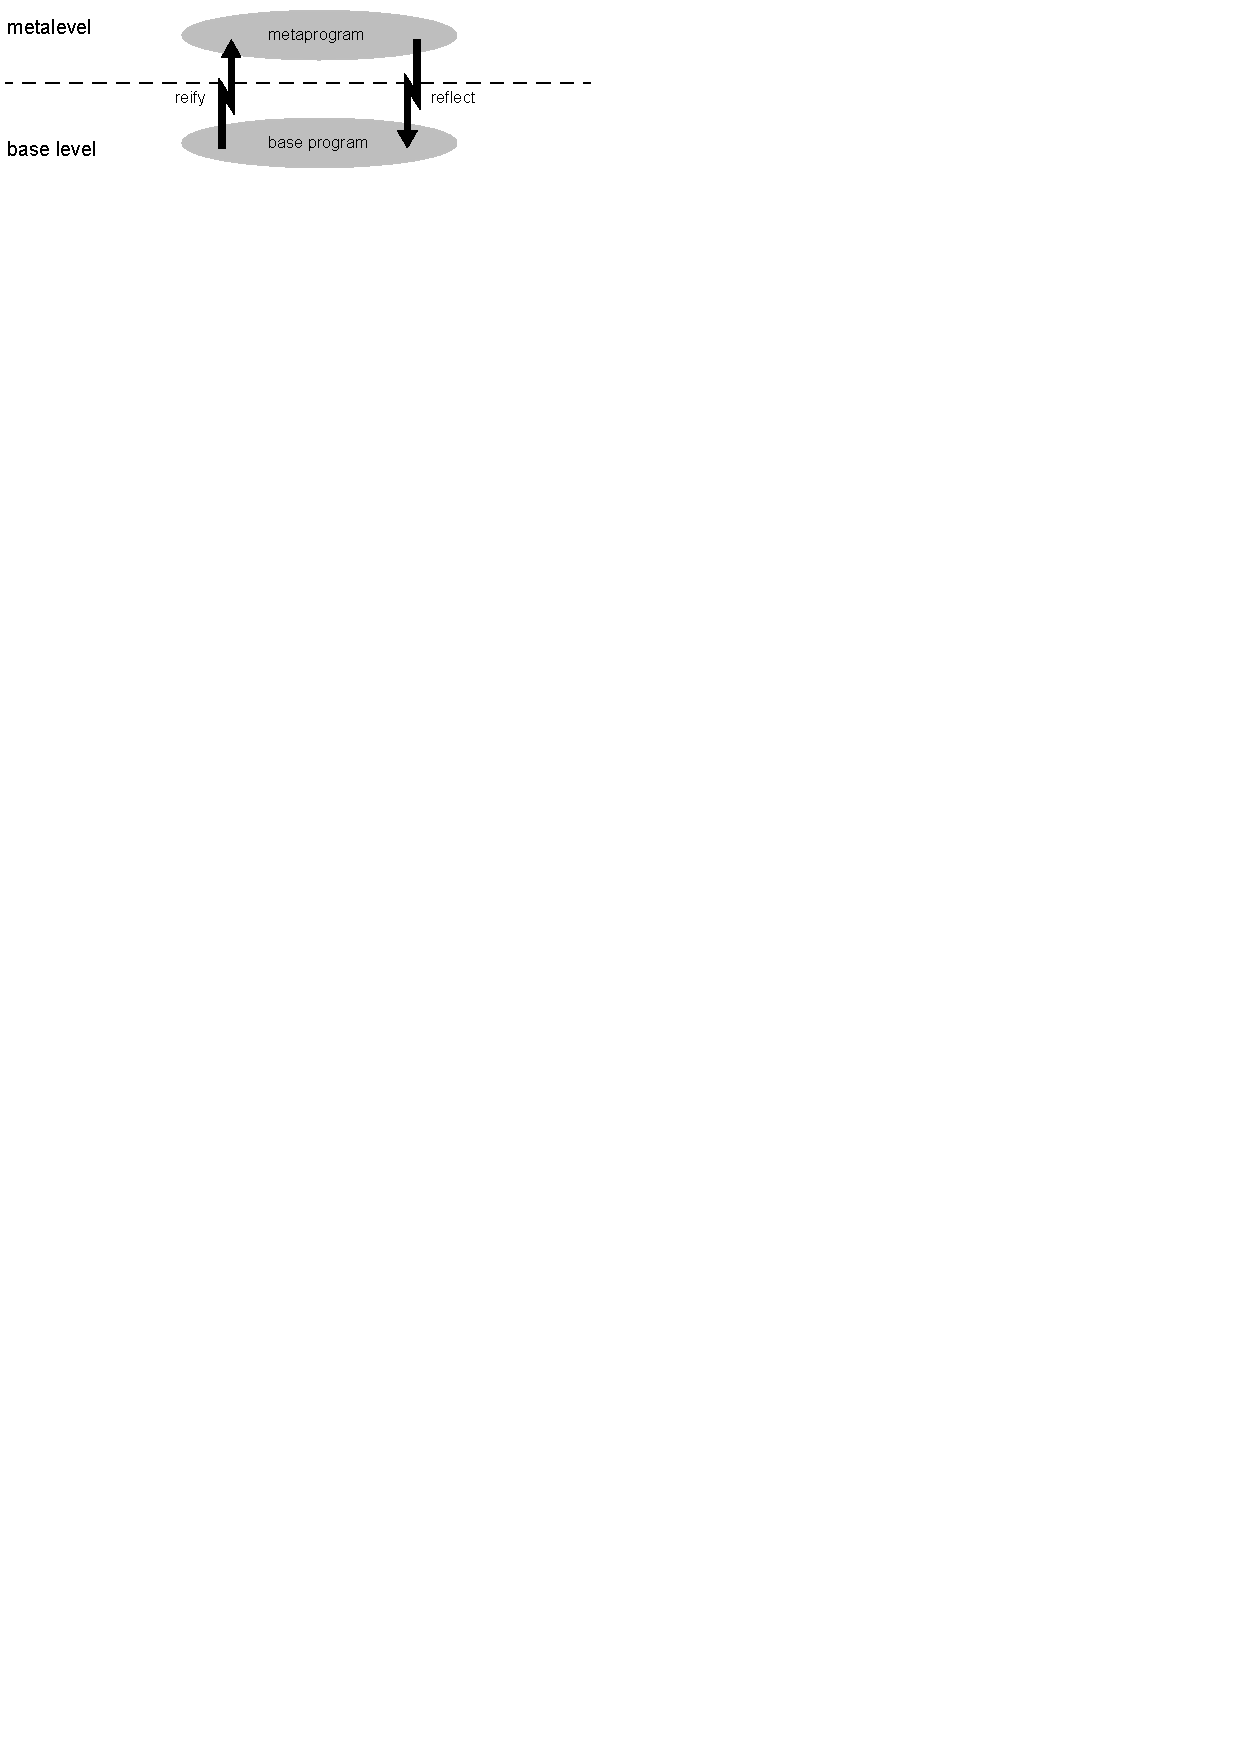
\includegraphics[trim=0 755 310 0, clip=true]{wand.pdf}
	 	\end{block}
	 	\pause
	 	\begin{block}{Operações}
	 	\begin{description}[reificação]
	 				\item [reificação] Obtém uma representação do programa em execução;
	 				\item [reflexão] Reflete as modificações realizadas na representação.
	 			\end{description}
	 	\end{block}
	 \end{frame}	  	 
  	 \begin{frame}{The Art of Metaobject Protocol \cite{kiczales1991art}}
  	 	\begin{block}{Descrição}
  	 		Descreve a implementação do protocolo de metaobjetos do CLOS (Common Lisp Object System).
  	 	\end{block}
  	 	\pause
  	 	\begin{block}{Protocolo de Metaobjetos}
  	 		\begin{itemize}
  	 			\item É a interface para acesso aos metaobjetos de um sistema (semelhante ao conceito de protocolo de Smalltalk);
  	 			\pause
  	 			\item Dependente de linguagem ($\neq$ Metamodelo UML);  
  	 			\pause
  	 			\item Operações podem ser agrupadas em dois grupos:
  	 			\pause
  	 			\begin{description}[Introspecção]  	 			
  	 				\item [Introspecção] Examinam a estrutura e estado;
  	 				\pause
  	 				\item [Intercessão] Realizam mudanças estruturais e comportamentais;
  	 			\end{description}
  	 		\end{itemize}
  	 	\end{block} 
  	 \end{frame}	
 	 \subsection{Introspecção}
 	 \begin{frame}{Introspecção}
 	 	\begin{block}{Definição -- \cite{forman2004java}}
 	 		É o ato de examinar a estrutura e o estado de um programa em execução.
 	 	\end{block}
 	 	\pause
 	 	\begin{block}{Suporte}
 	 		\begin{description}[Smalltalk:]
 	 			\item [Smalltalk:] Suporte nativo:
	 	 			\begin{itemize}
	 	 				\item \emph{Kernel-Classes} \& \emph{Kernel-Methods}.
	 	 			\end{itemize}
	 	 		\pause
 	 			\item [Java:] Suporte nativo: 
 	 			\begin{itemize}
	 	 			\item Pacote \emph{java.lang.reflect.*}; \\ 
	 	 			\item \emph{java.lang.Class} \& \emph{java.lang.StackTraceElement}.
 	 			\end{itemize}
 	 			\pause
 	 			\item [C++:] Suporte nativo rudimentar: 
	 	 			\begin{itemize}
	 	 				\item \emph{typeid} e \emph{std::type\_info};
	 	 				\item Suporte com o uso de ferramentas e extensões (QTMetaObjectCompiler, OpenC++)
	 	 			\end{itemize}
 			\end{description}
 		\end{block}
 	 \end{frame}
 	 \begin{frame}{Introspecção -- Exemplos (Java)}
 	 	\begin{exampleblock}{Obtenção dos atributos de um objeto}
 	 		\lstinputlisting{examples/reflection-field.java}
 	 	\end{exampleblock}
 	 	\pause
 	 	\begin{exampleblock}{Obtenção do método que invocou o método corrente}
 	 		\lstinputlisting{examples/method-find.java}
 	 	\end{exampleblock}
 	 \end{frame}
 	 \subsection{Intercessão}
 	 \begin{frame}{Intercessão Estrutural}
 	 	\begin{block}{Definição \cite{chiba2000load}}
 	 		Permite o programador alterar a definição de uma classe, método ou atributo de um programa em execução.
 	 	\end{block} 
 	 	\pause
 	 	\begin{block}{Suporte}
 	 		\begin{description}[Smalltalk:]
 	 			\item [Smalltalk:] Suporte nativo (usado pelo compilador);
 	 			\pause
 	 			\item [C++:] Sem suporte nativo:  
 	 				\begin{itemize}
		 	 			\item A extensão OpenC++ \cite{chiba1995metaobject} dá suporte;
		 	 		\end{itemize}
	 	 		\pause
 	 			\item [Java:] Suporte nativo limitado:
	 	 			\begin{itemize}
	 	 				\item \emph{Dynamic proxies} (\emph{java.lang.reflect.Proxy});
	 	 				\item Biblioteca Javassist \cite{chiba2000load} dá suporte;
	 	 			\end{itemize}
 	 		\end{description}
 	 	\end{block}
 	 \end{frame}
 	 \begin{frame}{Intercessão Estrutural -- Exemplos}
 	 	\begin{exampleblock}{Nova classe -- Smalltalk}
 	 		\lstinputlisting[otherkeywords={subclass:,instanceVariableNames:, classVariableNames:,poolDictionaries:,category:,\#MCDiffyVersion}]{examples/reflection-smalltalk.st}
 	 	\end{exampleblock}
 	 	\pause
 	 	\begin{exampleblock}{Dynamic Proxy -- Java}
 	 		\lstinputlisting{examples/dynamic-proxy.java}
 	 	\end{exampleblock}
 	 \end{frame}
 	 \begin{frame}{Intercessão Comportamental}
 	 	\begin{block}{Definição \cite{denker2008sub}}
 	 		Permite que a alteração de construtos relativos à execuçao de um programa (Ex. passagens de mensagens, acesso à variáveis)
 	 	\end{block} 
 	 	\pause		 	 	 	
 		\begin{block}{Suporte}
 			\begin{description}  [Smalltalk:] 
	 			\item [CLOS:] É a única linguagem com suporte nativo;
	 			\pause
	 			\item [Smalltalk:] Sem suporte nativo: 
	 			\begin{itemize}
	 				\item Persephone e Geppetto \cite{marschall2006taking,rothlisberger2006geppetto}.
	 			\end{itemize}
	 			\pause
	 			\item [Java:] Sem suporte nativo:
	 			\begin{itemize}
	 				\item Reflex e Javassit \cite{tanter2001reflex,chiba2000load}.
	 			\end{itemize}
	 		\end{description}
 	 	\end{block} 	 	 	 	
 	 \end{frame}
 	 \begin{frame}[c]{Intercessão Comportamental -- Exemplos}
 	 		\centering
 	 		\LARGE Será dado um exemplo prático mais adiante.
 	 \end{frame}
 	 \subsection{Críticas}
 	 \begin{frame}{Críticas à Programação Reflexiva}
 	 	\begin{block}{Perigoso}
 	 		\begin{quote}
 	 			Yes, you bet it is ! \\
 	 			Yes, if you're not careful. \\
 	 			Yes, but you can make it safer. \\
 	 			Yes, but so is crossing the street.
 	 			\begin{flushright}
 	 				Brian Foote
 	 			\end{flushright}
 	 		\end{quote}
 	 		%http://www.laputan.org/talks/ss98/sld003.htm
 	 	\end{block}
 	 	\pause
 	 	\begin{block}{Encapsulamento}
 	 		Com reflexão, é trivial ignorar modificadores de acesso:
 	 		\lstinputlisting{examples/private-access.java}
 	 	\end{block}
 	 \end{frame}
	 \begin{frame}{Críticas à Programação Reflexiva}
 	 	\begin{block}{Princípio Aberto/Fechado}
 	 		Reflexão pode ferir o princípio Aberto/Fechado  	 	 \cite{meyer1988object} -- é trivial ignorar restrições e modificar trechos de código originalmente fechados à modificação.
 	 	\end{block}
 	 	\pause
 	 	\begin{block}{Desempenho}
 	 		\begin{itemize}
 	 			\item Invocações via reflexão costumam ter um custo de invocação maior -- \alert{questão de implementação};
 	 		\end{itemize}
 	 		\footnotesize
 	 			\begin{table}[h]
 	 				\begin{tabular}{rcc}
 	 					& Normal (ms)              & Reflexão (ms)            \\
 	 					\hline \hline
 	 					Acesso a Atributos    & 57                  & 12585                \\
 	 					Chamada de Métodos    & 41                  & 901                  \\
 	 					Construção de Objetos & 121                 & 212                  \\ \hline
 	 					\multicolumn{3}{l}{\footnotesize{Fonte : \citeonline{janPetedi2008Reflexive}}}
 	 				\end{tabular}
 	 			\end{table} 	 
 	 	\end{block}
 	 \end{frame}
 	 \subsection{Melhores práticas}
	 \begin{frame}{Melhores práticas}
	 	\alert{Escrever}
 	 \end{frame}
 	\section{Exemplo Prático}
	 \begin{frame}{Open C++}
	 	\begin{block}{História}
			Criado em 1995 por Shigeru Chiba.
 	 	\end{block}
 	 	\pause
	 	\begin{block}{Motivação}
			\begin{itemize}
 	 			\item Fácil implementação de reflexão em C++
 	 			\pause
 	 			\item Possibilidade de criar códigos de otimização customizados
 	 			\pause
				\item Extensão não-intrusiva de reuso de código
 	 		\end{itemize}
 	 	\end{block}
	 \end{frame}
	 \begin{frame}{Open C++ - Exemplo}
 	 	\begin{block}{Adição de comportamento}
 	 		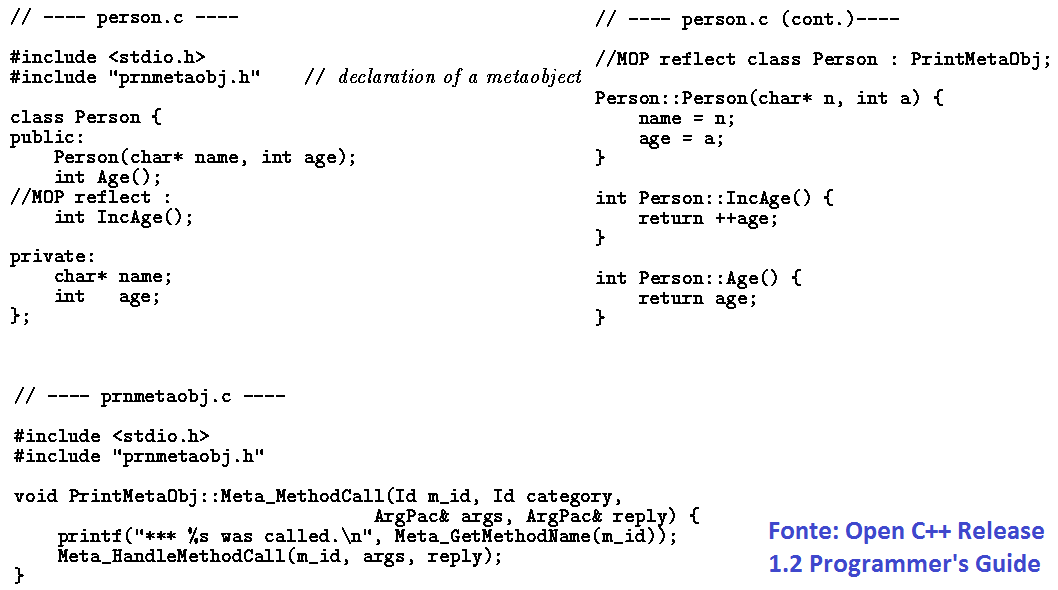
\includegraphics[width=1\textwidth]{examples/example_open_cxx}
 	 	\end{block}
	 \end{frame}
	 \begin{frame}{Javassist -- \textbf{Java} Programming A\textbf{ssist}ant}
	 	\begin{block}{História}
	 		\begin{itemize}
	 			\item Também criado por Shigeru Chiba \cite{chiba2000load};
	 			\pause
	 			\item Atualmente mantido pela JBoss;
	 			\pause
	 			\item Última versão -- 3.19.0-GA (06/01/2015).
	 		\end{itemize}
 	 	\end{block}
 	 	\pause
 	 	\begin{block}{Disponível em :}
			\url{http://jboss-javassist.github.io/javassist/}		
 	 	\end{block} 	 	
 	 	\pause
	 	\begin{block}{Características}
			\begin{itemize}
				\item Introspecção;
				\item Intersseção estrutural (\alert{classes não carregadas});
				\item Intersseção comportamental (\alert{com proxy e method handler});
 	 		\end{itemize}
 	 	\end{block}
	 \end{frame}
	 \begin{frame}{Javaassist}
	 	\begin{block}{Alguns projetos que usam}
	 		\begin{itemize}
	 			\item Hibernate;
	 			\item JBoss Seam;
	 		\end{itemize}
	 	\end{block}
	 	\pause
	 	\begin{exampleblock}{Decorador \cite{gamma1994design} reflexivo}
	 		\centering Exemplo prático na IDE
	 	\end{exampleblock}
	 	%\begin{exampleblock}{Observer on steroids}
 		%\end{exampleblock}
	 			 	
	 \end{frame}
 %	 	\begin{exampleblock}{Alteração de Super Classe}
 %	 		\lstinputlisting{examples/super-class.java}
 %	 	\end{exampleblock}
% 	 	\pause
% 	 	\begin{exampleblock}{Adição de comportamento}
% 	 		\lstinputlisting{examples/add-behavior.java}
% 	 	\end{exampleblock} 
%	 \end{frame}
%	 \begin{frame}{Easymock}
%	 	Mostrar o conceito de dynamic proxies do java (nativo)
%	 	Mostrar como é implementado. 
%	 	Fazer um paralelo com uma implementação em smalltalk, onde tem reflection ''de verdade'';
%	 \end{frame}
% \section{Trabalhos Atuais}	 
% \begin{frame}{Trabalhos Atuais}
% 	\alert{Escrever}
% \end{frame}
 \section{Referências}
 \begin{frame}[allowframebreaks]{Referências}
   \bibliography{apresentacao}
  \end{frame}
\end{document}

